% Figure 1. (a) the frame every session boots into, at native 320x200 scaled
% losslessly; (b) the movement axes, which run along screen diagonals.
% Grid: 1 unit = 1 cm. Panel (a) spans (0,0)-(9.4,5.875), panel (b)
% (10.0,0)-(14.6,5.875). Layers: L0 panels, L1 axes, L2 labels.
\documentclass[tikz,border=1pt]{standalone}
\usepackage{times}
\usepackage[T1]{fontenc}
\usetikzlibrary{arrows.meta,calc}
% so the figure builds from paper/src as well as from paper/src/figures
\graphicspath{{.}{figures/}}

\definecolor{ink}{HTML}{1C1C1E}
\definecolor{soft}{HTML}{9C9C9F}
\definecolor{accent}{HTML}{2F6FB0}
\definecolor{tile}{HTML}{F2F3F5}
\definecolor{rule}{HTML}{DCDDE0}
\definecolor{wash}{HTML}{E8F0F8}

\begin{document}
\begin{tikzpicture}[
  font=\sffamily,
  >={Stealth[length=2.5mm,width=1.8mm]},
  axis/.style={draw=accent,line width=1.0pt,->},
  keylab/.style={font=\sffamily\small\bfseries,text=accent,inner sep=1.5pt},
  alias/.style={font=\sffamily\scriptsize,text=ink,inner sep=1.2pt},
  panel/.style={font=\sffamily\small\bfseries,text=ink},
  note/.style={font=\sffamily\scriptsize,text=soft,align=center},
]
% ================= panel (a): the opening frame =========================
\node[inner sep=0,anchor=south west] (frame) at (0,0)
  {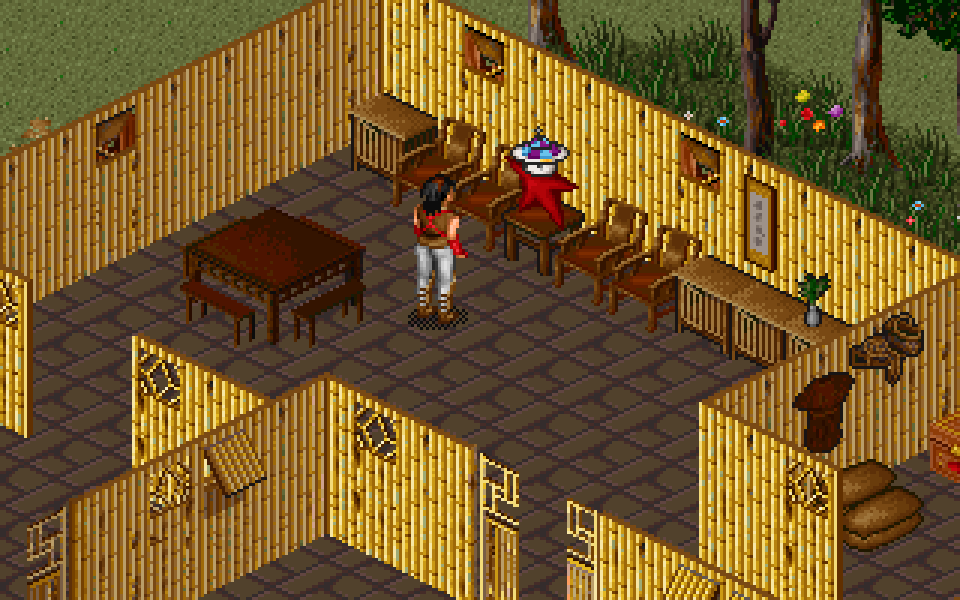
\includegraphics[width=9.4cm]{opening.png}};
\draw[rule,line width=0.5pt] (0,0) rectangle (9.4,5.875);
\node[panel,anchor=north west] at (0,-0.14) {(a)};
\node[note,anchor=north west,align=left] at (0.52,-0.12)
  {the frame every session boots into, $320\times200$, upscaled without interpolation};

% ================= panel (b): the movement axes =========================
\begin{scope}[shift={(10.0,0)}]
  \fill[tile] (0,0) rectangle (4.6,5.875);
  \draw[rule,line width=0.5pt] (0,0) rectangle (4.6,5.875);
  \coordinate (P) at (2.3,2.94);

  % isometric tile field, 3x3 diamonds around the centre
  \foreach \i in {-1,0,1}{\foreach \j in {-1,0,1}{
    \fill[white,draw=rule,line width=0.4pt]
      ($(P)+({(\i-\j)*0.66},{(\i+\j)*0.33})+(-0.66,0)$)
      -- ++(0.66,0.33) -- ++(0.66,-0.33) -- ++(-0.66,-0.33) -- cycle;}}
  \fill[wash,draw=accent,line width=0.7pt]
    ($(P)+(-0.66,0)$) -- ++(0.66,0.33) -- ++(0.66,-0.33) -- ++(-0.66,-0.33) -- cycle;
  \fill[accent] (P) circle (2.0pt);

  % start clear of the player tile, stop clear of the labels
  \foreach \sx/\sy/\ex/\ey in {-0.40/0.20/-1.24/0.62, 0.40/0.20/1.24/0.62,
                              -0.40/-0.20/-1.24/-0.62, 0.40/-0.20/1.24/-0.62}
    \draw[axis] ($(P)+(\sx,\sy)$) -- ($(P)+(\ex,\ey)$);

  \node[keylab,anchor=south east] at ($(P)+(-1.30,0.68)$) {kp7};
  \node[alias,anchor=north east]  at ($(P)+(-1.26,0.64)$) {left};
  \node[keylab,anchor=south west] at ($(P)+(1.30,0.68)$)  {kp9};
  \node[alias,anchor=north west]  at ($(P)+(1.26,0.64)$)  {up};
  \node[keylab,anchor=north east] at ($(P)+(-1.30,-0.68)$){kp1};
  \node[alias,anchor=south east]  at ($(P)+(-1.26,-0.64)$){down};
  \node[keylab,anchor=north west] at ($(P)+(1.30,-0.68)$) {kp3};
  \node[alias,anchor=south west]  at ($(P)+(1.26,-0.64)$) {right};

  \node[note,anchor=north] at (2.3,5.62)
    {the four keys that move the character,\\each aliasing one arrow key};
  \node[note,anchor=south] at (2.3,0.26)
    {no key walks straight up\\or straight across the screen};
  \node[panel,anchor=north west] at (0,-0.14) {(b)};
\end{scope}
\end{tikzpicture}
\end{document}
